\usetikzlibrary{arrows}
\usetikzlibrary{shapes.geometric, arrows}

%\definecolor{Gcolor}{HTML}{3b528b}
%\definecolor{Dcolor}{HTML}{e41a1c}

%\definecolor{Gcolor}{HTML}{2c7fb8}
%\definecolor{Dcolor}{HTML}{f03b20}

\definecolor{Gcolor}{HTML}{2c7fb8}
\definecolor{Dcolor}{HTML}{f03b20}

\tikzstyle{generator} = [thick, rectangle, rounded corners, minimum width=1.5cm, minimum height=1cm,text centered, draw=Gcolor]
\tikzstyle{discriminator} = [thick, rectangle, rounded corners, minimum width=1.5cm, minimum height=1cm,text centered, draw=Dcolor]
\tikzstyle{mmd} = [thick, rectangle, rounded corners, minimum width=1.5cm, minimum height=1cm,text centered, draw=black]
\tikzstyle{io} = [thick,circle, trapezium left angle=70, trapezium right angle=110, minimum width=1.2cm, minimum height=1cm, text centered, draw=black]

\tikzstyle{iodotted} = [thick, circle, trapezium left angle=70, trapezium right angle=110, minimum width=1.2cm, minimum height=1cm, text centered, draw=black, dotted]

\tikzstyle{process} = [thick, rectangle, minimum width=1cm, minimum height=1cm, text centered, draw=black]

\tikzstyle{xG} = [thick,rectangle, minimum width=2.2cm, minimum height=3cm, text depth= 2.2cm, draw=black]
\tikzstyle{s0} = [thick,rectangle, minimum width=2cm, minimum height=3cm, text centered]
\tikzstyle{s1} = [thick, dotted, rectangle, minimum width=1.6cm, minimum height=1.1cm, text centered, draw=black]


\tikzstyle{decision} = [thick,rectangle, minimum width=1cm, minimum height=1cm, text centered, draw=black]


\tikzstyle{dots} = [circle, minimum size=2pt, inner sep=0pt,outer sep=0pt, draw=Dcolor, fill = Dcolor]

\tikzstyle{arrow} = [thick,->,>=stealth]

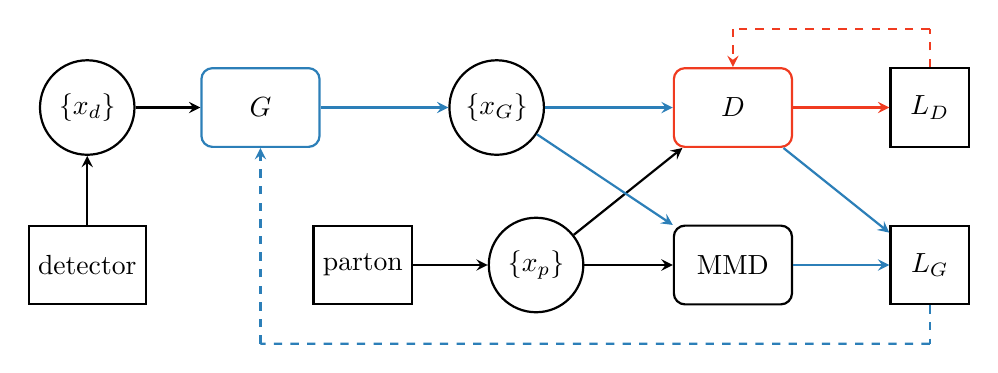
\begin{tikzpicture}[node distance=2cm]


\node (generator) [generator] {$G$};
\node (xG) [io, right of = generator, xshift=1.0cm, yshift=0cm] {$\{x_G\}$};
\node (xd) [io, left of=generator, xshift=-0.2cm, yshift=0cm] {$\{x_d\}$};
\node (discriminator) [discriminator, right of = xG, xshift=1.0cm, yshift=0cm] {$D$};

\node (xp) [io, below of = xG, xshift=0.5cm, yshift=0cm] {$\{x_p\}$};

\node (detector) [process, below of=xd, xshift=-0.0cm, yshift=0cm] {detector};
\node (parton) [process, left of=xp, xshift=-0.2cm, yshift=0cm] {parton};

\draw [arrow, color=black] (detector) -- (xd);
\draw [arrow, color=black] (parton) -- (xp);
\draw [arrow, color=black] (xd) -- (generator);
\draw [arrow, color=black] (xp) -- (discriminator);
\draw [arrow, color=Gcolor] (generator) -- (xG);
\draw [arrow, color=Gcolor] (xG) -- (discriminator);

\node (dloss) [process, right of=discriminator, xshift=0.5cm, yshift=0cm] {$L_{D}$};
\node (gloss) [process, below of=dloss, xshift=0.0cm, yshift=0cm] {$L_{G}$};
\node (mmd) [mmd, below of=discriminator, xshift=0.0cm, yshift=0cm] {MMD};

\draw [arrow, color=Gcolor] (discriminator) -- (gloss);
\draw [arrow, color=Dcolor] (discriminator) -- (dloss);

\coordinate[ above of = dloss, xshift=0cm, yshift=-1cm] (d1);
\coordinate[ above of = discriminator, xshift=0cm, yshift=-1cm] (d2);
\draw[thick, dashed, color=Dcolor] (dloss) -- (d1);
\draw[thick, dashed, color=Dcolor] (d1) -- (d2);
\draw[arrow, dashed, color=Dcolor] (d2) -- (discriminator);

\draw[arrow, color=Gcolor] (xG) --  (mmd);
\draw[arrow, color=black] (xp) --  (mmd);
\draw[arrow, color=Gcolor] (mmd) --  (gloss);


\coordinate[ below of = gloss, xshift=0cm, yshift=1.0cm] (out1);
\coordinate[ below of = generator, xshift=0cm, yshift=-1.0cm] (out2);
\draw[thick, dashed, color=Gcolor] (gloss) --  (out1);
\draw[thick, dashed, color=Gcolor] (out1) --  (out2);
\draw[arrow, dashed, color=Gcolor] (out2) --  (generator);








\end{tikzpicture}
